\chapter{Calibration}
The calibration process is based on the linear method \cite{Tsai1988} with some application specific modifications. In the following the method will be described and the modifications will be discussed. 


\subsection{Notation}
In the formulation of hand-eye calibration a number of homogeneous transforms between different frames will be described. Most literature uses a mathematical notation of A\textit{i}, B\textit{i}, A, B, X and Y leading to a clean expression. In this work a more engineering friendly and explicit notation will be used stating for each transform the pose index, the frame described and the reference frame. Examples of the notation are given in table \ref{tab:notation}. The transform represents a 4x4 matrix containing a 3x3 rotation matrix and a 3D translation vector. \\

\begin{table}[h]
\caption{Examples of the notation.}
\begin{tabular}{ll}
\label{tab:notation}
$[T_{i}]_{camera}^{object}$   & The transform from object to camera at the \textit{i}th view           \\[8pt] 
$[T_{i}]_{base}^{TCP}$        & The transform from end-effector to base at the \textit{i}th view       \\[8pt] 
$[T_{i}]_{TCP}^{camera}$      & The transform from camera to end-effector at the \textit{i}th view     \\[8pt] 
$[T_{i-1,i}]_{camera}$        & The camera frame of pose \textit{i} relative to the camera frame of pose \textit{i-1}  \\[8pt]              
\end{tabular}
\end{table}

\begin{figure}[htb]
	\begin{center}
		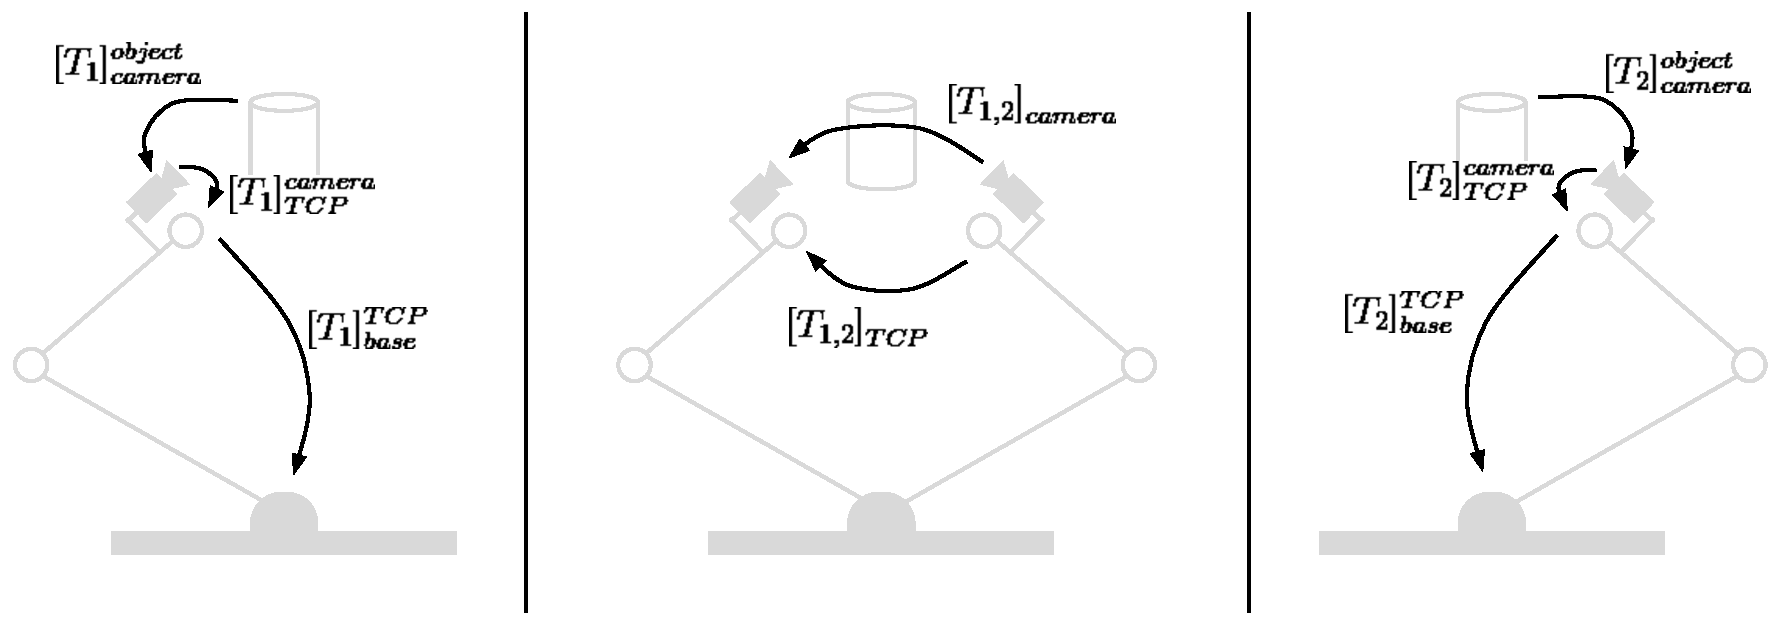
\includegraphics[width=\textwidth,trim=0 0 0 0]{graphics/03_calibration/hand_eye_transforms.pdf}%trim=l b r t
		\caption{Sketch of a robot with a camera mounted on the end-effector in two different poses capturing a cylinder object. Shows the robot in pose 1 (left), pose 2 (right) and both poses in same image (center).}\label{fig:hand_eye_transforms}
		
	\end{center}
\end{figure}

\subsection{Linear hand-eye calibration}
\noindent Looking at figure \ref{fig:hand_eye_transforms} it is clear that a kinematic chain from object to the robot base can be formulated (\ref{fig:hand_eye_transforms}, left and right).\\

\begin{equation}
	[T_{i}]_{base}^{object} = [T_{i}]_{base}^{TCP} \cdot [T_{i}]_{TCP}^{camera} \cdot [T_{i}]_{camera}^{object}
\end{equation} \\

\noindent The transform from end-effector to robot base can be found from the joint states of the robot and the transform from object to camera can, assuming the camera is calibrated, be found from projection geometry. This leaves only the transform from camera to end-effector as unknown. Assuming that the object is static and captured from different poses of the robot, it is possible to formulate the transform between the two camera poses (\ref{fig:hand_eye_transforms}, center).\\

\begin{equation}\label{eq:object_camera}
\begin{matrix}
[T_{1,2}]_{camera} \cdot [T_{1}]_{camera}^{object} = [T_{2}]_{camera}^{object} \\
\\  
\Updownarrow \\ 
\\ 
[T_{1,2}]_{camera} = [T_{2}]_{camera}^{object} \cdot ([T_{1}]_{camera}^{object})^{-1}
\end{matrix}
\end{equation}\\ 

\noindent Similarly the transform between the two poses of the end-effector can be formulated(\ref{fig:hand_eye_transforms}, center).\\

\begin{equation}
\begin{matrix}
[T_{1}]_{base}^{TCP} \cdot [T_{1,2}]_{TCP} = [T_{2}]_{base}^{TCP} \\ 
\\ 
\Updownarrow \\ 
\\ 
[T_{1,2}]_{TCP} = ([T_{2}]_{base}^{TCP})^{-1} \cdot  [T_{1}]_{base}^{TCP}
\end{matrix}
\end{equation}\\ 

\noindent Assuming that the transform from camera to end-effector is static it is clear that.\\

\begin{equation}
[T_{1}]_{TCP}^{camera} = [T_{2}]_{TCP}^{camera} = [T]_{TCP}^{camera}
\end{equation}\\ 

\noindent This makes it possible to formulate a closed loop kinematic chain (in most literature denoted $ AX=XB $).\\

\begin{equation} \label{equ:closed_loop}
	[T_{1,2}]_{camera} \cdot [T]_{TCP}^{camera} = [T]_{TCP}^{camera} \cdot [T_{1,2}]_{TCP}
\end{equation}\\ 

\noindent The missing transform can thus be found by solving a set of $ n-1 $ linear equations for $ n $ poses \\

\begin{equation}
\left\{\begin{matrix}
[T_{1,2}]_{camera} \cdot [T]_{TCP}^{camera} = [T]_{TCP}^{camera} \cdot [T_{1,2}]_{TCP} \\ 
\ \ \vdots 
\\ 
[T_{i-1,i}]_{camera} \cdot [T]_{TCP}^{camera} = [T]_{TCP}^{camera} \cdot [T_{i-1,i}]_{TCP}\\ 
\ \ \vdots 
\\ 
[T_{n-1,n}]_{camera} \cdot [T]_{TCP}^{camera} = [T]_{TCP}^{camera} \cdot [T_{n-1,n}]_{TCP}
\end{matrix}\right.
\end{equation}\\ 

\noindent Normally the calibration is made by capturing several poses of a chessboard marker and yields good results. There are however two rather implicit assumptions \cite{Horaud1995} not justified by this approach. First the calibration of the camera assumes a perfect pinhole model and that the optical axis of the camera is perpendicular to the object, but equation \ref{equ:closed_loop} assumes that the object is static, which for most practical objects are contradictions. There are several approaches to solving this, but most modern approaches combines camera calibration with hand-eye calibration. 

\marginnote{Refs} 









